\documentclass{article}
\usepackage{spconf,amsmath,amssymb,graphicx}
\usepackage{enumitem}
\setlist{nosep,leftmargin=14pt}
\usepackage{booktabs}
\usepackage{cite}
\usepackage{url}
\usepackage{tikz}
\usetikzlibrary{arrows.meta,positioning}

\title{GRAPH-INFORMED FLOW MATCHING FOR EEG RECONSTRUCTION UNDER CHANNEL LOSS}

\name{Author Name(s)}
\address{Department and Institution\\
City, Country\\
email@example.com}

\begin{document}
\maketitle

\begin{abstract}
Electroencephalography (EEG) reconstruction after electrode failure requires
recovering channel traces from remaining spatial and temporal context. We
implement graph-informed flow matching (GiFlow), which initializes a
conditional flow with a spatiotemporal heat-kernel estimate, and SRG-flow,
which adds residual-direction guidance and step-dependent velocity
calibration. We evaluate both under 50\% whole-channel loss on
participant-disjoint DEAP-RAW and SEED-IV splits, aligning named electrodes
to a shared 62-channel space and fitting dataset-specific normalization on
training participants. In a matched single-seed pilot, joint GiFlow achieved
macro normalized mean-squared error (NMSE) 0.6127 and SRG-flow 0.6198,
compared with 0.6022 for K-nearest-neighbour (KNN) interpolation. Joint
training lowered NMSE relative to source-specific training in this split,
but also changed graph estimation. Neither learned model surpassed KNN in
macro NMSE. These preliminary findings require repeated seeds, additional
missingness patterns, and feature- or task-level evaluation.
\end{abstract}

\begin{keywords}
Electroencephalography, signal reconstruction, missing data, graph neural
networks, flow matching
\end{keywords}

\section{Introduction}

Electroencephalography (EEG) is recorded at spatially distributed electrodes.
When an electrode disconnects or fails, its entire temporal trace may be
lost, rather than a random collection of isolated samples. Reconstructing a
missing channel therefore requires using both cross-electrode relationships
and temporal structure. Simple spatial interpolation provides a useful
reference, but its performance can depend on the observed electrode
configuration and does not learn a reconstruction trajectory from data.

Flow matching offers a way to learn such a trajectory. A vector field is
trained to transport samples along a prescribed path between a source
distribution and the target distribution \cite{lipman2023flow}. GiFlow
instantiates this idea for spatiotemporal imputation by constructing its
source with graph heat kernels, then learning a vector field over a linear
path toward the complete signal \cite{zhang2026giflow}. This is particularly
relevant to EEG, where electrodes form a spatial system and adjacent time
samples have a natural temporal neighbourhood.

Recent EEG spatial super-resolution work, including step-aware
residual-guided diffusion (SRGDiff), uses step-dependent residual cues to
steer reconstruction \cite{liu2026srgdiff}. SRGDiff is a latent diffusion
method; it is not itself a flow-matching model. We therefore implement
SRG-flow as a separate adaptation of its residual-guidance and modulation
ideas to GiFlow's continuous flow path, without introducing a VAE or a
diffusion noise-prediction objective.

This paper documents the current implementation and its completed
participant-held-out pilot. DEAP-RAW and SEED-IV differ in electrode
coverage, signal scale, and acquisition protocol
\cite{koelstra2012deap,zheng2019emotionmeter}. We align named electrodes in
a shared channel space, keep absent channels distinct from observed zeros,
and fit normalization separately for each dataset. The central comparison
tests GiFlow and SRG-flow against KNN and feature-propagation baselines under
50\% whole-channel loss.

The paper makes three limited contributions. First, it describes an
end-to-end implementation with data alignment, training-only graph
estimation, adaptive graph filtering, masked flow matching, and Euler
inference. Second, it specifies a matched joint-versus-individual
participant-held-out comparison on raw DEAP and SEED-IV data. Third, it
reports the resulting single-seed measurements without claiming superiority:
joint training lowered learned-model NMSE in this split, but KNN remained
stronger on macro NMSE. Broader conclusions require repeated seeds and the
additional evaluations described in the limitations.

\section{Methodology}

\subsection{Task Definition and Data Masks}

Let $X \in \mathbb{R}^{N \times R}$ be a complete EEG window with $N$
electrodes and $R$ time samples. Let $O \in \{0,1\}^{N \times R}$ mark
genuinely recorded measurements, $M$ the conditioning mask supplied to the
model, and $Q$ the artificial evaluation mask. They satisfy
$M \odot Q=0$ and $M+Q\leq O$, where $\odot$ denotes elementwise
multiplication. The model receives
$X_{\mathrm{cond}}=M\odot X$ and is scored only on entries selected by $Q$.
Naturally absent samples and padded electrodes are excluded from scoring.
At inference, observed entries are restored exactly after integration.

The primary task hides half of the available electrode traces
($\rho=0.5$). Evaluation masks are sampled in canonical electrode-name order,
ensuring the same named channels are hidden in the matched joint and
individual runs. During training, a conditioning submask is generated by
retaining a randomly sampled fraction in $[0.3,0.9]$ of available entries,
with an additional 0.5 probability of dropping each electrode for an
example. The code also implements point, contiguous-block, and synchronized
stream-outage masks; these conditions have not yet been included in the
reported real-data comparison.

\subsection{Datasets, Alignment, and Splits}

DEAP-RAW BioSemi BDF recordings are read using the 32 named EEG electrodes
and resampled to 200~Hz \cite{koelstra2012deap}. SEED-IV is loaded from raw
MATLAB trial recordings with its 62-channel electrode order and trial
boundaries retained \cite{zheng2019emotionmeter}. Channel names are
canonicalized before mapping both sources into a shared 62-electrode space.
An electrode not present in a source is zero-padded in the aligned tensor
and marked absent with a node-presence mask; it is never treated as an
observed zero-valued measurement.

Each source has its own standard scaler, fitted using the training split
only. Predictions are transformed back to the corresponding source scale
before evaluation. Thus signal-scale differences do not enter the
cross-source macro NMSE calculation.

The bounded pilot used 25 evenly selected, non-overlapping windows of
100 samples per participant. Splits were participant-disjoint. SEED-IV
participants 7, 10, and 15 were assigned to the fixed test split, and DEAP
participants 03, 05, 11, 12, 22, and 26 formed its test split; remaining
participants were assigned deterministically to training and validation.
In joint training, the two datasets were sampled with equal probability.
The participant split, window selection, evaluation masks, training budget,
and inference settings were matched between GiFlow and SRG-flow.

\subsection{Spatial and Temporal Graphs}

The spatial graph for each source is estimated from training windows only,
so held-out participants do not contribute to graph construction. For
electrode signals $x_i$ and $x_j$, the implementation calculates their
absolute correlation $|r_{ij}|$, defines distance
$d_{ij}=1-|r_{ij}|$, and applies the Gaussian weight
\begin{equation}
    w_{ij}=\exp\left[-(d_{ij}/\omega)^2\right],
\end{equation}
where $\omega$ is the standard deviation of off-diagonal distances. Weights
below 0.1 are removed and the remaining adjacency is binary. For joint
training, the two source graphs are averaged edgewise only when both
electrodes occur in that source. The temporal graph is a line graph joining
successive samples. The resulting spatial and temporal Laplacians define
the heat-kernel prior; normalized adjacency operators are used by the
message-passing layers.

\subsection{Graph-Informed Flow Prior}

For spatial and temporal Laplacians $L_s$ and $L_t$, respectively, GiFlow
initializes the trajectory with
\begin{equation}
    X_0 =
    \exp(-\tau_s L_s)(M \odot X)\exp(-\tau_t L_t),
    \label{eq:prior}
\end{equation}
where $\tau_s$ and $\tau_t$ control spatial and temporal smoothing. The
filtering factors are fitted on training windows by minimizing the
signal-alignment and spatial-smoothness objective
\begin{equation}
    \mathcal{L}_{\tau} =
    \mathbb{E}\left[
    \|X-X_0\|_2^2 +
    \alpha_{\tau}\operatorname{tr}(X_0^\top L_s X_0)
    \right].
    \label{eq:tau}
\end{equation}
They are frozen before vector-field training and inference. The pilot did
not impose a positive lower bound on either factor; a tau-floor sweep is
not yet complete.

\subsection{Conditional Flow-Matching Network}

For a sampled flow time $t\sim\mathcal{U}(0,1)$, GiFlow defines a linear
path and constant target velocity:
\begin{align}
    X_t &= (1-t)X_0+tX, \\
    U_t &= X-X_0.
\end{align}
The vector field is conditioned on the current state $X_t$, visible signal
$X_{\mathrm{cond}}$, mask $M$, and a flow-time embedding. A learned node
embedding is propagated over the electrode graph and used by spatial
attention. Temporal attention operates over the $R$ samples at each
electrode, with positional encodings. The fused features pass through
spatiotemporal propagation, which alternates spatial and temporal graph
message passing, and an output multilayer perceptron predicts a velocity
for each electrode-time pair.

For training target mask $T$, the masked velocity loss is
\begin{equation}
    \mathcal{L}_{\mathrm{flow}} =
    \frac{\|T\odot
    [v_{\theta}(X_t,X_{\mathrm{cond}},M,t)-U_t]\|_2^2}
    {\max(\|T\|_1,1)}.
    \label{eq:flow}
\end{equation}
An observed-value preservation loss uses the one-step endpoint estimate
$\widetilde{X}=X_t+(1-t)v_{\theta}$:
\begin{equation}
    \mathcal{L}_{\mathrm{pres}} =
    \frac{\|M\odot(\widetilde{X}-X)\|_2^2}
    {\max(\|M\|_1,1)}.
\end{equation}
The GiFlow training objective is
$\mathcal{L}_{\mathrm{flow}}+
\lambda_{\mathrm{pres}}\mathcal{L}_{\mathrm{pres}}$.

\subsection{SRG-Flow Residual and Modulation}

SRG-flow retains the GiFlow prior, flow path, and base vector field. It
adds a residual-direction module $r_{\phi}$ and a step-aware modulation
module predicting scale $\gamma_t$ and bias $\beta_t$. At each flow time,
the corrected velocity is
\begin{equation}
    v'_t =
    \gamma_t\left(v_{\theta}+
    \lambda_{\mathrm{res}}r_{\phi}\right)+\beta_t.
    \label{eq:srg}
\end{equation}
The residual target is
$U_t-\operatorname{stopgrad}(v_{\theta})$ and is scored on $T$. The
modulation loss penalizes $(\gamma_t-1)^2+\beta_t^2$, encouraging the
correction to remain close to identity calibration unless data support a
change. The SRG-flow objective adds weighted residual-regression and
modulation terms to the flow and preservation losses. This adaptation does
not use SRGDiff's VAE, latent diffusion, or noise-prediction objective.

\subsection{Training and Inference}

Training proceeds in two stages. First, the filtering factors are optimized
on training windows and frozen. Second, the vector field is trained with
Adam, and an exponential moving average (EMA) of the weights is evaluated
on validation NMSE for checkpoint selection. The matched pilot used hidden
dimension 64, four spatiotemporal propagation layers, dropout 0.1, batch
size 32, learning rate $10^{-3}$, weight decay $5\times 10^{-5}$,
preservation weight 0.1, and a maximum of 50 epochs with patience 8.
Filtering-factor optimization ran for 20 epochs. SRG-flow used
$\lambda_{\mathrm{res}}=1$ and $\lambda_{\mathrm{smm}}=0.01$. No tau floor
was used. All six runs were performed on an NVIDIA RTX 4050. Inference used
a deterministic 10-step Euler solver:
\begin{equation}
    X^{(k+1)}=X^{(k)}+\Delta t\,v_{t_k}(X^{(k)}),
    \qquad \Delta t=1/10,
\end{equation}
with $v_{t_k}=v_{\theta}$ for GiFlow and $v_{t_k}=v'_t$ for SRG-flow.
Observed samples are restored exactly after the final step.

\subsection{Implemented Ablation Controls}

Beyond the two learned models in the real-data comparison, the codebase
includes a Gaussian-source flow baseline, spatial-only and temporal-only
prior variants, and switches that disable spatial attention, temporal
attention, or spatiotemporal propagation. It also exposes point, block,
whole-channel, and shared-stream masks; spatial and temporal tau floors;
per-step observed-value clamping; prior renormalization; and normalized
Laplacians. These controls make targeted ablations possible, but they are
not reported as completed real-data comparisons here. The synthetic
smoke tests check that selected control combinations execute; they are not
evidence of reconstruction quality.

\begin{figure*}[t]
\centering
\resizebox{\textwidth}{!}{%
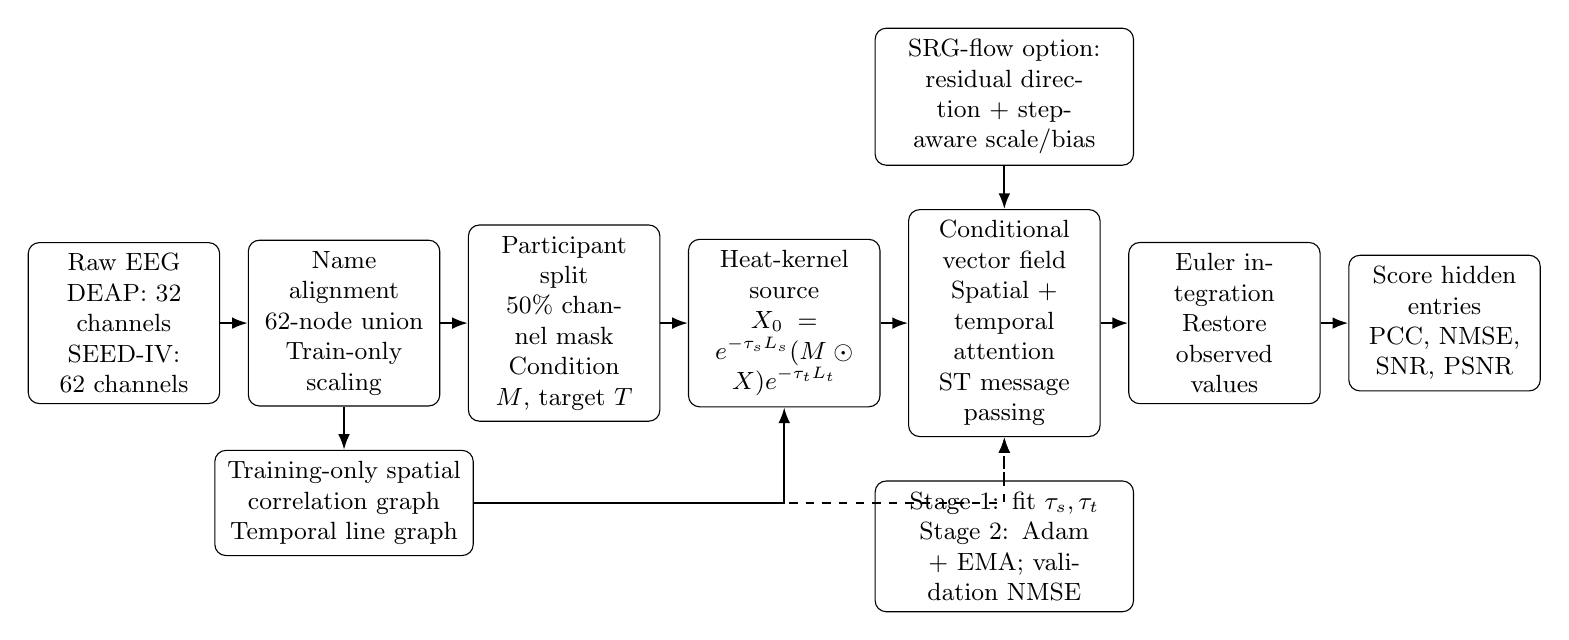
\begin{tikzpicture}[
    >=Latex,
    node distance=0.35cm,
    block/.style={draw, rounded corners, align=center, minimum height=1.15cm,
                  text width=2.15cm, inner sep=4pt, font=\small},
    aux/.style={draw, rounded corners, align=center, minimum height=0.85cm,
                text width=3.0cm, inner sep=4pt, font=\small},
    arrow/.style={-{Latex[length=2mm]}, thick},
    trainarrow/.style={-{Latex[length=2mm]}, thick, dashed}
]
\node[block] (data) {Raw EEG\\DEAP: 32 channels\\SEED-IV: 62 channels};
\node[block, right=of data] (align) {Name alignment\\62-node union\\Train-only scaling};
\node[block, right=of align] (mask) {Participant split\\50\% channel mask\\Condition $M$, target $T$};
\node[block, right=of mask] (prior) {Heat-kernel source\\$X_0=e^{-\tau_sL_s}(M\odot X)e^{-\tau_tL_t}$};
\node[block, right=of prior] (field) {Conditional vector field\\Spatial + temporal attention\\ST message passing};
\node[block, right=of field] (solve) {Euler integration\\Restore observed values};
\node[block, right=of solve] (score) {Score hidden entries\\PCC, NMSE, SNR, PSNR};
\node[aux, below=0.55cm of align] (graphs) {Training-only spatial correlation graph\\Temporal line graph};
\node[aux, below=0.55cm of field] (fit) {Stage 1: fit $\tau_s,\tau_t$\\Stage 2: Adam + EMA; validation NMSE};
\node[aux, above=0.55cm of field] (srg) {SRG-flow option:\\residual direction + step-aware scale/bias};
\draw[arrow] (data) -- (align);
\draw[arrow] (align) -- (mask);
\draw[arrow] (mask) -- (prior);
\draw[arrow] (prior) -- (field);
\draw[arrow] (field) -- (solve);
\draw[arrow] (solve) -- (score);
\draw[arrow] (align) -- (graphs);
\draw[arrow] (graphs) -| (prior);
\draw[trainarrow] (graphs) -| (field);
\draw[trainarrow] (fit) -- (field);
\draw[arrow] (srg) -- (field);
\end{tikzpicture}%
}
\caption{Implemented data and model workflow. Solid arrows show the
reconstruction path; dashed arrows indicate training-time graph and
optimization information. SRG-flow adds residual guidance and affine
modulation to the GiFlow velocity.}
\label{fig:pipeline}
\end{figure*}

\section{Experimental Protocol}

\subsection{Comparison Conditions}

Six single-seed runs form the matched comparison: joint GiFlow and SRG-flow,
DEAP-only GiFlow and SRG-flow, and SEED-IV-only GiFlow and SRG-flow. Each
uses the same participant split, 25 windows per participant, 50\%
whole-channel evaluation loss, 50\% training channel-drop probability,
batch size, filtering-factor budget, epoch cap, and 10-step inference.
Graphs are estimated from training windows; the joint models use the
pairwise-averaged graph, while the individual models use the graph of their
source. Thus joint-versus-individual is a whole-pipeline comparison and
does not isolate the effect of adding training examples alone.

KNN spatial interpolation and feature propagation (FP) are the principal
non-learned references. Spatial mean, temporal mean, and linear
interpolation are also implemented as baselines; results are shown in the
comparison plot. All methods are evaluated on the same hidden entries for
each source. The joint test split contains 240,000 scored entries for
DEAP-RAW and 232,500 for SEED-IV-MAT.

\subsection{Metrics}

Metrics are calculated only on artificially hidden, genuinely available
entries. For predictions $\widehat{X}$ and reference values $X$, the primary
error measure is
\begin{equation}
    \mathrm{NMSE}=
    \frac{\sum Q\odot(\widehat{X}-X)^2}
    {\sum Q\odot X^2}.
\end{equation}
PCC is computed over the scored entries. Signal-to-noise ratio (SNR) is
$10\log_{10}\left(\sum Q\odot X^2/
\sum Q\odot(\widehat{X}-X)^2\right)$. PSNR uses the range of scored
reference values divided by RMSE. MAE and RMSE are retained in source
units, but are not macro-averaged across datasets because DEAP and SEED-IV
have different signal scales. The joint macro NMSE and macro PCC are the
arithmetic means of the two source-specific pooled scores.

\section{Results}

\subsection{Joint and Source-Specific Model Comparison}

Table~\ref{tab:models} reports pooled test NMSE and PCC, the learned
filtering factors and validation-selected epoch are reported in
Table~\ref{tab:filtering}. For joint training, Table~\ref{tab:models} also
reports macro NMSE. Table~\ref{tab:baselines}
compares the joint learned models with the strongest non-learned references
from the matched joint run.

\begin{table*}[t]
\centering
\caption{Participant-held-out 50\% channel-loss results from the matched
single-seed study. Lower NMSE is better; higher PCC is better. Individual
training is reported only on its training source.}
\label{tab:models}
\small
\begin{tabular}{llccc}
\toprule
Training & Model & DEAP-RAW NMSE / PCC & SEED-IV-MAT NMSE / PCC & Macro NMSE\\
\midrule
Joint & GiFlow    & 0.5920 / 0.6261 & 0.6333 / 0.6313 & 0.6127\\
Joint & SRG-flow  & 0.5979 / 0.6219 & 0.6416 / 0.6248 & 0.6198\\
\midrule
DEAP only & GiFlow   & 0.6325 / 0.5942 & -- & --\\
DEAP only & SRG-flow & 0.8456 / 0.4247 & -- & --\\
SEED-IV only & GiFlow   & -- & 0.7571 / 0.5351 & --\\
SEED-IV only & SRG-flow & -- & 0.7216 / 0.5409 & --\\
\bottomrule
\end{tabular}
\end{table*}

\begin{table*}[t]
\centering
\caption{Validation-selected epoch and fitted heat-kernel factors for each
single-seed run. Epoch numbering is zero-based.}
\label{tab:filtering}
\small
\begin{tabular}{llccc}
\toprule
Training & Model & Epoch & $\tau_s$ & $\tau_t$\\
\midrule
Joint & GiFlow & 2 & 0.0194 & 0.0381\\
Joint & SRG-flow & 2 & 0.0193 & 0.0469\\
DEAP only & GiFlow & 40 & 2.5104 & 0.0528\\
DEAP only & SRG-flow & 2 & 2.5685 & 0.0543\\
SEED-IV only & GiFlow & 2 & 0.0476 & 0.0882\\
SEED-IV only & SRG-flow & 3 & 0.0466 & 0.0792\\
\bottomrule
\end{tabular}
\end{table*}

\begin{table*}[t]
\centering
\caption{Joint-run comparison with non-learned baselines. Values are shown
as source-specific NMSE / PCC and PSNR / SNR (dB).}
\label{tab:baselines}
\small
\setlength{\tabcolsep}{3pt}
\begin{tabular}{lccccc}
\toprule
Method & DEAP N / P & SEED-IV N / P &
DEAP PSNR / SNR & SEED-IV PSNR / SNR & Macro N\\
\midrule
GiFlow & 0.5920 / 0.6261 & 0.6333 / 0.6313 & 26.08 / 2.28 & 31.90 / 1.98 & 0.6127\\
SRG-flow & 0.5979 / 0.6219 & 0.6416 / 0.6248 & 26.04 / 2.23 & 31.84 / 1.93 & 0.6198\\
KNN & 0.5931 / 0.6258 & 0.6113 / 0.6258 & 26.07 / 2.27 & 32.06 / 2.14 & 0.6022\\
Feature propagation & 0.6052 / 0.6167 & 0.6506 / 0.5913 & 25.98 / 2.18 & 31.78 / 1.87 & 0.6279\\
\bottomrule
\end{tabular}
\vspace{2pt}
\parbox{\textwidth}{\small N: NMSE; P: PCC.}
\end{table*}

Joint GiFlow achieved the lowest learned-model NMSE on both sources:
0.5920 on DEAP-RAW and 0.6333 on SEED-IV-MAT. SRG-flow was slightly worse
on NMSE for both datasets, although its pooled PCC was close to GiFlow's.
KNN achieved the best macro NMSE (0.6022), lower than both joint learned
models. GiFlow narrowly improved over KNN on DEAP alone (0.5920 versus
0.5931), but not on SEED-IV (0.6333 versus 0.6113). SRG-flow did not
outperform KNN on either source. Feature propagation had macro NMSE 0.6279.
The gain of joint GiFlow over joint KNN on DEAP is small and should not be
interpreted as a reliable advantage from a single split.

The jointly trained runs scored 472,500 hidden test entries in total:
240,000 from the DEAP test participants and 232,500 from the SEED-IV test
participants. These counts describe the selected pilot windows and are
not independent subjects or repeated trials.

\begin{figure*}[t]
\centering
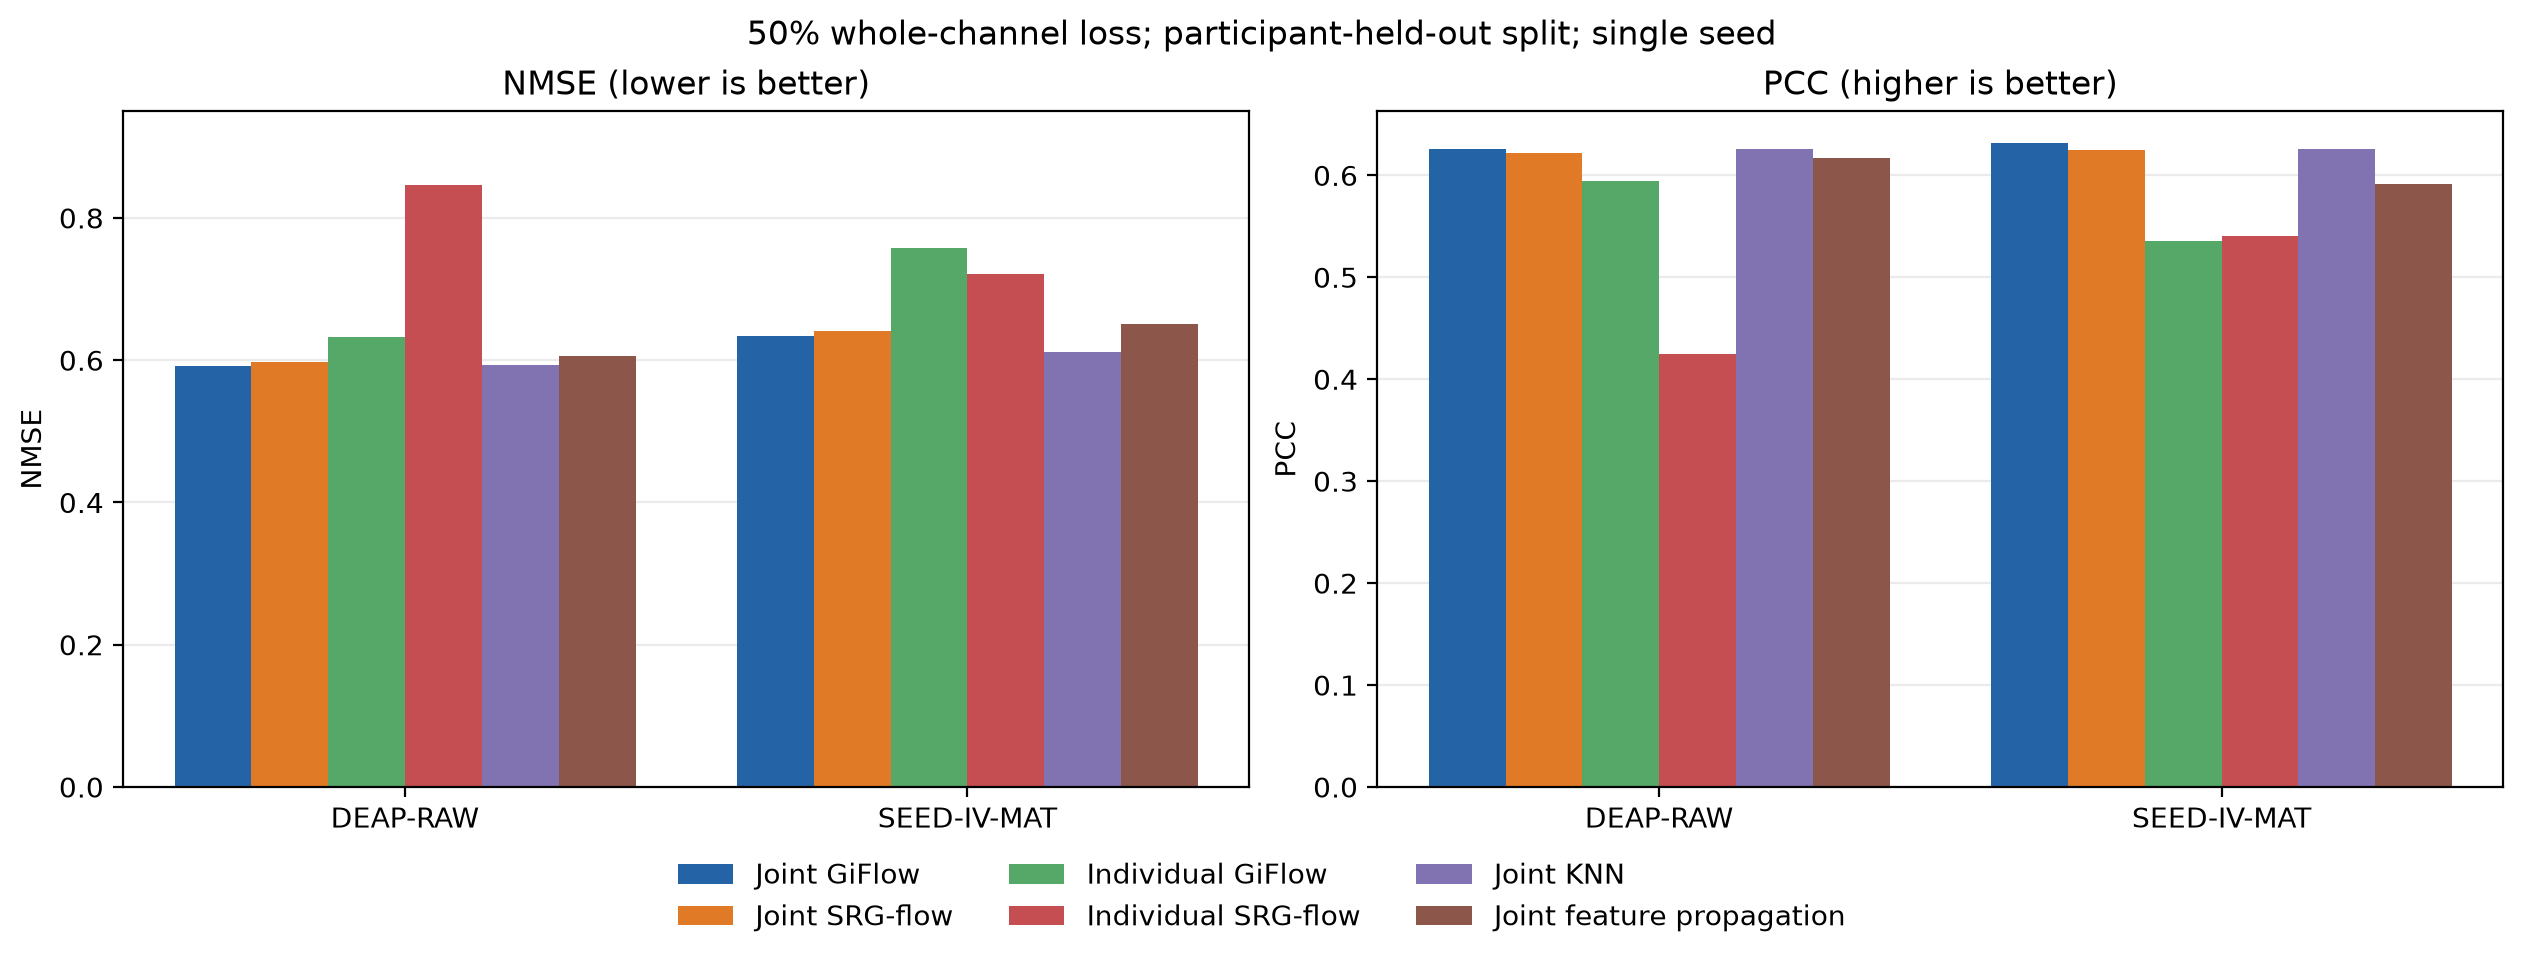
\includegraphics[width=0.94\textwidth]{figures/isbi2027_model_comparison.png}
\caption{Source-specific NMSE and PCC for joint and source-specific GiFlow
and SRG-flow, KNN, and feature propagation under 50\% whole-channel loss.
All bars are from the same participant-held-out seed-0 pilot; the figure
does not represent between-seed variability.}
\label{fig:jointresults}
\end{figure*}

\begin{figure*}[t]
\centering
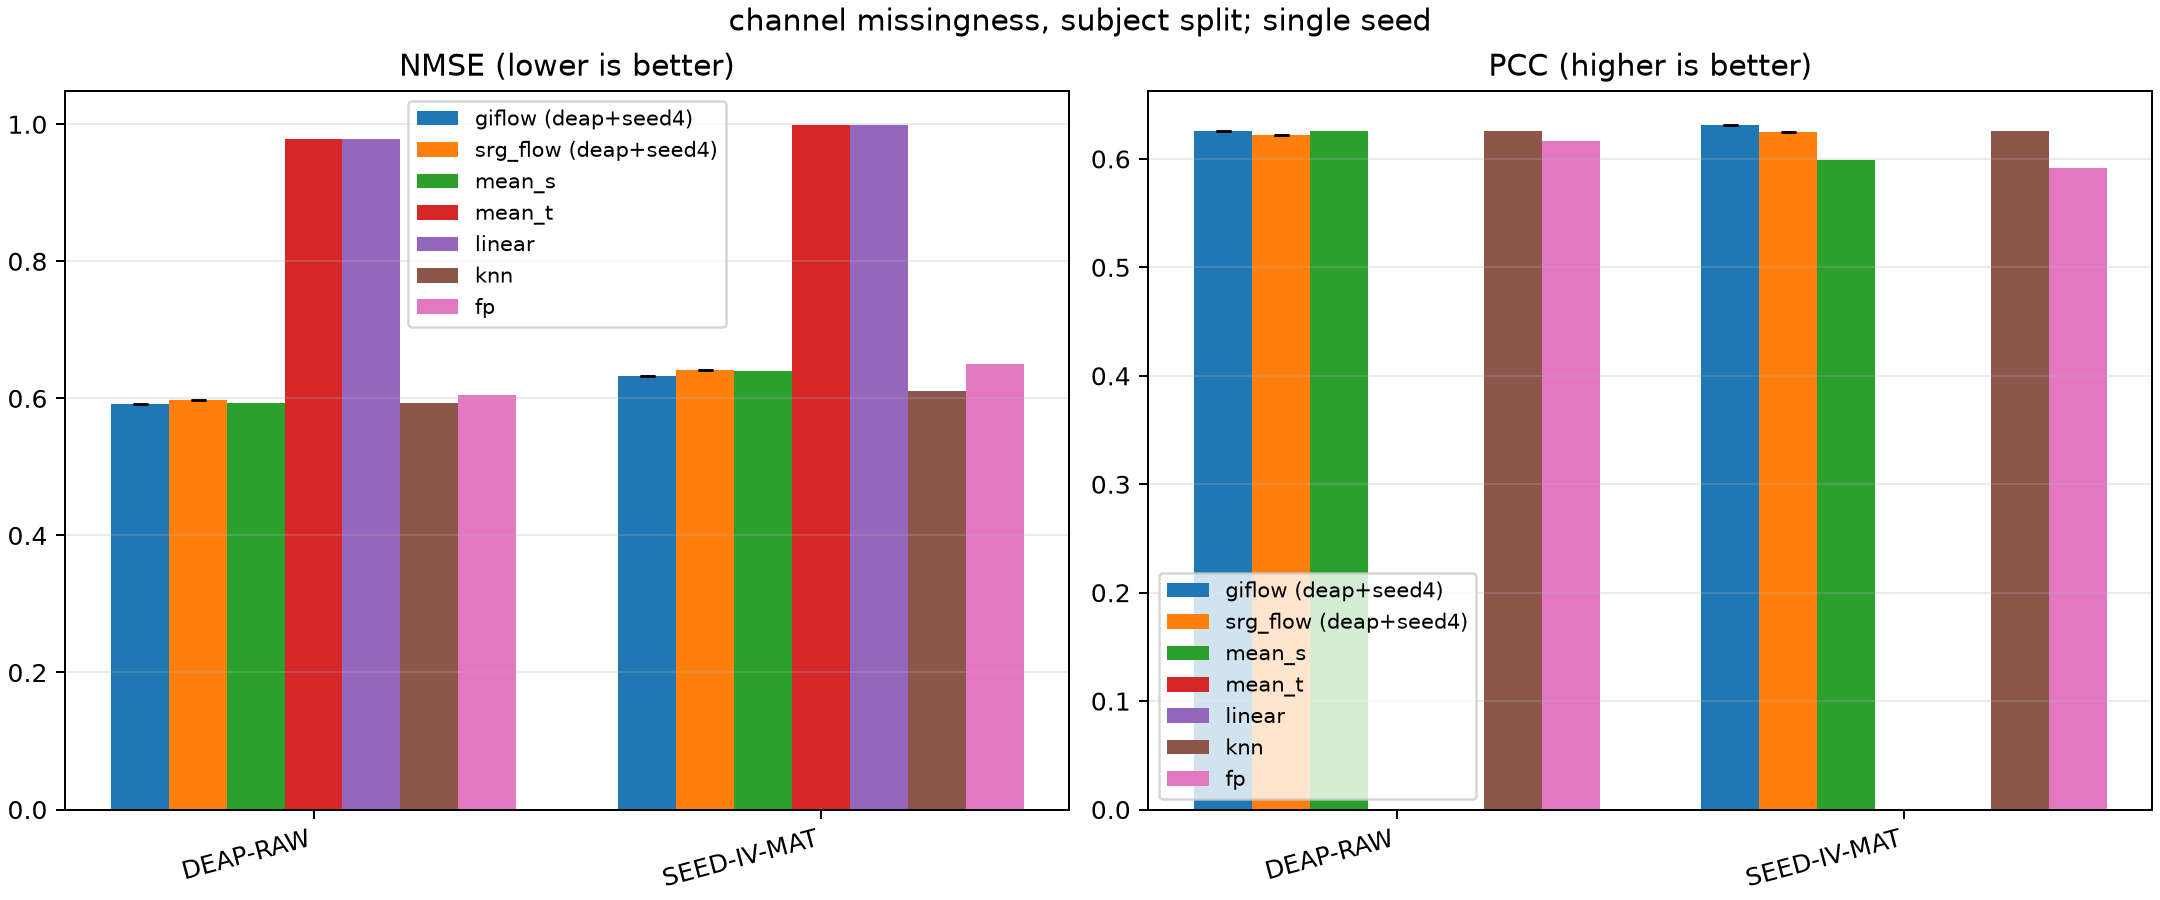
\includegraphics[width=0.94\textwidth]{figures/isbi2027_joint_comparison.png}
\caption{Additional joint-run baselines, including spatial mean, temporal
mean, and linear interpolation, compared with the learned models. The
near-zero PCC and high NMSE of the temporal and linear methods under
whole-channel loss reflect the absence of within-channel conditioning
samples for the hidden electrodes.}
\label{fig:allbaselines}
\end{figure*}

\subsection{Joint Versus Individual Training}

For both learned architectures, joint training was associated with lower
NMSE than source-specific training in this split. GiFlow NMSE decreased
from 0.6325 to 0.5920 on DEAP and from 0.7571 to 0.6333 on SEED-IV.
SRG-flow decreased from 0.8456 to 0.5979 on DEAP and from 0.7216 to
0.6416 on SEED-IV. These differences are descriptive: the joint models
use an averaged cross-source graph while individual models use
source-specific graphs, so this experiment changes both the training data
and the graph prior.

For context, source-specific KNN graph baselines achieved NMSE 0.5964 on
DEAP and 0.6097 on SEED-IV. They outperformed each corresponding
source-specific learned model in this pilot. These baseline values use
individual-source graphs and should not be conflated with the joint KNN
scores in Table~\ref{tab:baselines}. Source-scale MAE/RMSE for the joint
GiFlow, SRG-flow, and KNN runs were, respectively, 0.009442/0.028177,
0.009729/0.028316, and 0.009401/0.028201 on DEAP; and
10.6430/16.2994, 10.8282/16.4060, and 10.2885/16.0130 on SEED-IV.
These values are reported in each source's native scale and are not
aggregated across datasets.

\subsection{Participant Heterogeneity and Learned Smoothing}

Pooled scores conceal substantial participant-level variability. For joint
GiFlow, the equal-participant mean and standard deviation of PCC/NMSE were
0.124$\pm$0.421 / 0.691$\pm$0.477 for the six DEAP test participants and
0.618$\pm$0.131 / 0.639$\pm$0.145 for the three SEED-IV test participants.
For SRG-flow, the corresponding values were
0.115$\pm$0.409 / 0.754$\pm$0.531 and
0.610$\pm$0.137 / 0.648$\pm$0.165. The low DEAP participant-average PCC
and large dispersion indicate that performance is not uniform across
subjects, despite the more favourable pooled PCC.

The learned smoothing factors also differed by training regime. Joint
GiFlow used $\tau_s=0.0194$ and $\tau_t=0.0381$, while joint SRG-flow used
$\tau_s=0.0193$ and $\tau_t=0.0469$. Source-specific DEAP training
learned much larger spatial factors ($\tau_s=2.5104$ for GiFlow and
2.5685 for SRG-flow); source-specific SEED-IV training learned
$\tau_s=0.0476$ and 0.0466, respectively. These values motivate testing
tau floors, but do not establish that a floor improves performance.

\section{Discussion}

The current results do not support a claim that residual-guided flow
improves this reconstruction task: SRG-flow's macro NMSE (0.6198) was
higher than GiFlow's (0.6127), and its source-specific NMSE was also
higher in the matched joint run. Residual correction and step-aware
calibration are implemented and tested as a model variant, but their
utility remains an empirical question requiring controlled repeated
experiments.

KNN is a strong reference under 50\% channel removal. It has lower joint
macro NMSE than either learned model and remains competitive even on the
DEAP source where joint GiFlow is marginally better. This points to a
clear next step: improve the learned prior and training stability, while
retaining simple spatial interpolation as a required baseline. The large
DEAP participant dispersion further suggests that pooled metrics alone
are insufficient.

Several limitations constrain interpretation. All reported learned-model
comparisons use one random seed and a bounded selection of 25 windows per
participant. Point, block, and shared-stream missingness are implemented
but not yet evaluated in the real-data study. Spatial and temporal tau
floors have not been swept, and the pilot does not measure EEG-FID,
spectral or topographic reconstruction error, or downstream emotion-task
performance. The datasets have different recording scales and
acquisition protocols; separate normalization and source-specific
reporting reduce, but do not eliminate, this domain shift. Finally, the
joint-versus-individual comparison changes the graph as well as the
training data.

\section{Conclusion}

We presented the implemented GiFlow and SRG-flow pipelines for EEG
reconstruction under whole-electrode loss and evaluated them in a matched
single-seed participant-held-out pilot on DEAP-RAW and SEED-IV. Joint
training was associated with lower NMSE than source-specific training,
but the comparison is confounded by differences in the estimated graph.
KNN interpolation achieved lower macro NMSE than either learned model,
and SRG-flow did not improve over GiFlow in the matched joint condition.
These measurements are preliminary rather than final performance claims.
Repeated-seed comparisons, additional corruption patterns, tau-floor
ablations, and feature- or task-level evaluation are needed to determine
whether learned flow reconstruction offers a robust advantage for EEG
channel recovery.

\section*{Compliance with Ethical Standards}
This study uses previously collected EEG datasets. [Authors: verify the
applicable dataset licenses and institutional requirements, and replace
this note with the required ethics/compliance statement before submission.]

\section*{Acknowledgments}
An AI assistant using Copilot SDK in VS Code was used to draft the Abstract,
Introduction, Methodology, Results, Discussion, and Conclusion. The authors
must verify and edit this material and are responsible for the final
manuscript. [Authors: add funding and conflict-of-interest statements here.]

\bibliographystyle{IEEEbib}
\bibliography{isbi2027_references}

\end{document}
